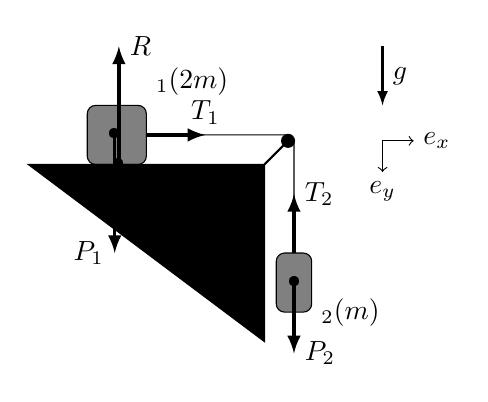
\begin{tikzpicture} [
	scale=.75,
	force/.style={->,>=latex,draw=\JRLblue,very thick,nodes={\JRLblue}},
	plane/.style={draw=\JRLblueC,fill=\JRLblueC},
	vecteur/.style={-latex,thick},
	] 
	% blocs
	\draw[fill=gray,rounded corners=3pt] (-3,0) rectangle (-2,1) node[above right]{$\ptB_1 (2m)$}; 
	\draw[fill=gray,rounded corners=3pt](0.2,-1.5)rectangle (0.8,-2.5)node[right]{$\ptB_2 (m)$}; 
	% support	
	\draw[plane] (-4,0)-|(0,-3)--cycle;
	\draw[\JRLblueF] (-4,0)-|(0,-3);
	
	% fil
	\draw[rounded corners=3pt] (-2,0.5) --(0.5,0.5)--++(0,-2) ; 	
	\draw[thick,fill] (0,0)--(0.4,0.4) circle(0.1); 
	% forces
	\draw[force](-2,.5)--+(1,0)node[above]{$\vv{T_1}$};
	\draw[force](.5,-1.5)--+(0,1)node[right]{$\vv{T_2}$};
	\draw[force](.5,-2)node{•}--+(0,-1.2)node[right]{$\vv{P_2}$};
	\draw[force,shift={(-1pt,0)}](-2.5,.5)node{•}--+(0,-2)node[left]{$\vv{P_1}$};
	\draw[force,shift={(1pt,0)}](-2.5,0)node{•}--+(0,2)node[right]{$\vv{R}$};	
	\draw[vecteur,shift={(2,2)}] (0,0)--+(0,-1) node[midway,right]{$\vv{g}$};	
	% base
	\draw[<->,shift={(2,0.4)}](15pt,0)node[right]{$\vv{e_x}$}-|(0pt,-15pt)node[below]{$\vv{e_y}$};
\end{tikzpicture}